\section{699 --- Falling Squares}
On an infinite number line ($x$-axis), we drop given squares in the order they are given.

The $i$-th square dropped (\lstinline[language=C++, basicstyle=\small\ttfamily, keywordstyle=\bfseries\color{green!40!black}]|positions[i] = (left, side_length)|) is a square with the left-most point being \lstinline[language=C++, basicstyle=\small\ttfamily, keywordstyle=\bfseries\color{green!40!black}]|positions[i][0]| and sidelength \lstinline[language=C++, basicstyle=\small\ttfamily, keywordstyle=\bfseries\color{green!40!black}]|positions[i][1]|.

The square is dropped with the bottom edge parallel to the number line, and from a higher height than all currently landed squares. We wait for each square to stick before dropping the next.

The squares are infinitely sticky on their bottom edge, and will remain fixed to any positive length surface they touch (either the number line or another square). Squares dropped adjacent to each other will not stick together prematurely.

Return a list of heights, $H$. Each height $H[i]$ represents the current highest height of any square we have dropped, after dropping squares represented by \lstinline[language=C++, basicstyle=\small\ttfamily, keywordstyle=\bfseries\color{green!40!black}]|positions[0], positions$[1]|, $\ldots$, \lstinline[language=C++, basicstyle=\small\ttfamily, keywordstyle=\bfseries\color{green!40!black}]|positions[i]|.


\paragraph{Example 1:}
\begin{flushleft}
\textbf{Input}:

\lstinline[language=C++, basicstyle=\small\ttfamily, keywordstyle=\bfseries\color{green!40!black}]|[[1, 2], [2, 3], [6, 1]]|

\textbf{Output}: \lstinline[language=C++, basicstyle=\small\ttfamily, keywordstyle=\bfseries\color{green!40!black}]|[2, 5, 5]|

\textbf{Explanation}:

After the first drop of positions \lstinline[language=C++, basicstyle=\small\ttfamily, keywordstyle=\bfseries\color{green!40!black}]|[0] = [1, 2]|:

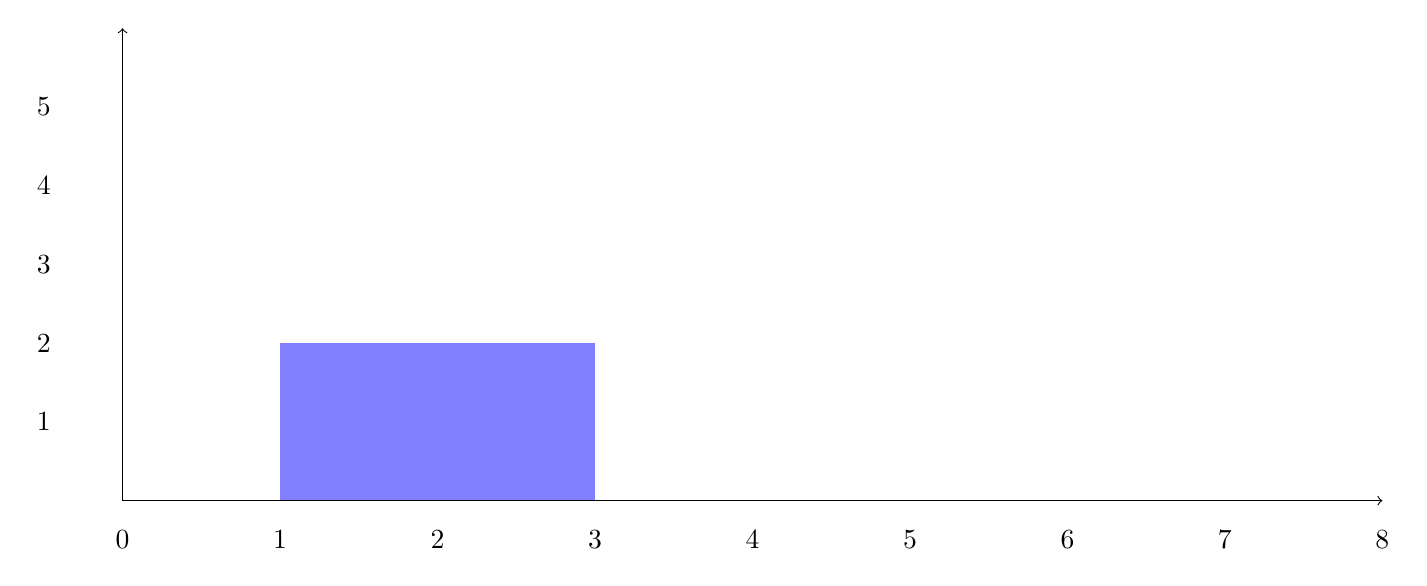
\begin{tikzpicture}
\fill[color=blue!50] (3,0.5cm) rectangle ++(4,2cm);
\draw[->] (1,0.5cm) -- ++(16,0);
\draw[->] (1,0.5cm) -- ++(0,6cm);
\foreach \x / \y in {1/0,3/1,5/2,7/3, 9/4, 11/5, 13/6, 15/7, 17/8}
\node (\x) at (\x, 0) {$\y$};
\foreach \x / \y in {1.5cm/1, 2.5cm/2, 3.5cm/3, 4.5cm/4, 5.5cm/5}
\node (\x) at (0, \x) {$\y$};
\end{tikzpicture}

The maximum height of any square is 2.

After the second drop of positions \lstinline[language=C++, basicstyle=\small\ttfamily, keywordstyle=\bfseries\color{green!40!black}]|[1] = [2, 3]|:
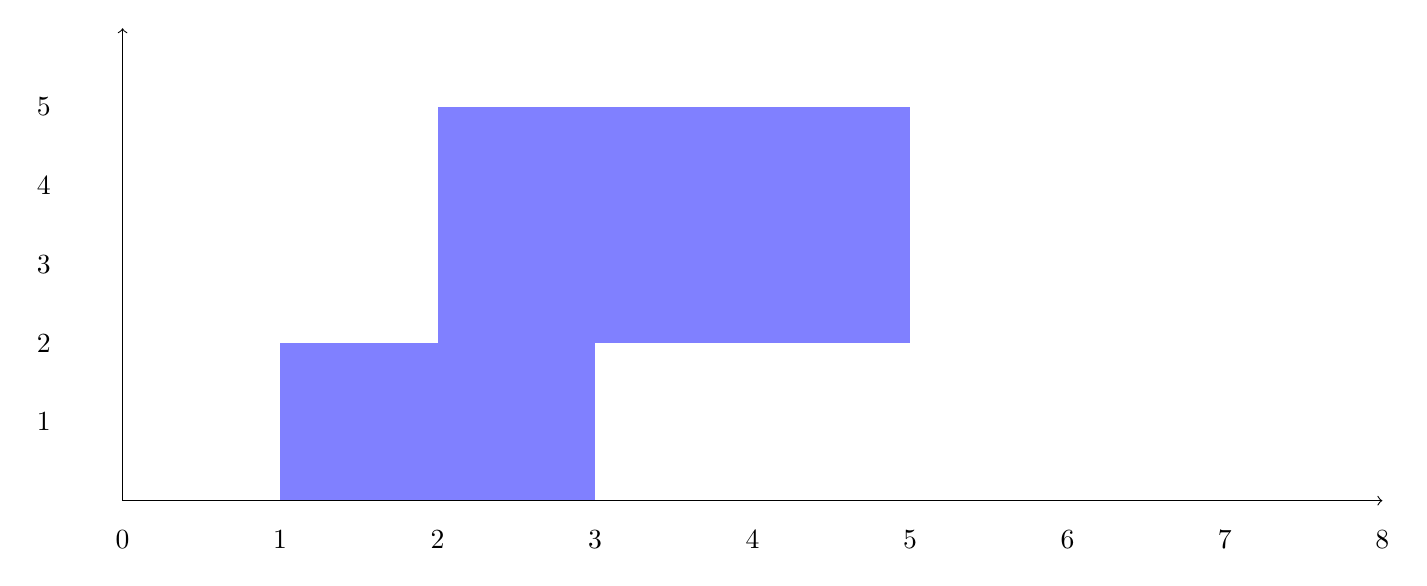
\begin{tikzpicture}
\fill[color=blue!50] (5,2.5cm) rectangle ++(6,3cm);
\fill[color=blue!50] (3,0.5cm) rectangle ++(4,2cm);
\draw[->] (1,0.5cm) -- ++(16,0);
\draw[->] (1,0.5cm) -- ++(0,6cm);
\foreach \x / \y in {1/0,3/1,5/2,7/3, 9/4, 11/5, 13/6, 15/7, 17/8}
\node (\x) at (\x, 0) {$\y$};
\foreach \x / \y in {1.5cm/1, 2.5cm/2, 3.5cm/3, 4.5cm/4, 5.5cm/5}
\node (\x) at (0, \x) {$\y$};
\end{tikzpicture}

The maximum height of any square is 5.  

The larger square stays on top of the smaller square despite where its center of gravity is, because squares are infinitely sticky on their bottom edge.

After the third drop of positions \lstinline[language=C++, basicstyle=\small\ttfamily, keywordstyle=\bfseries\color{green!40!black}]|[1] = [6, 1]|:
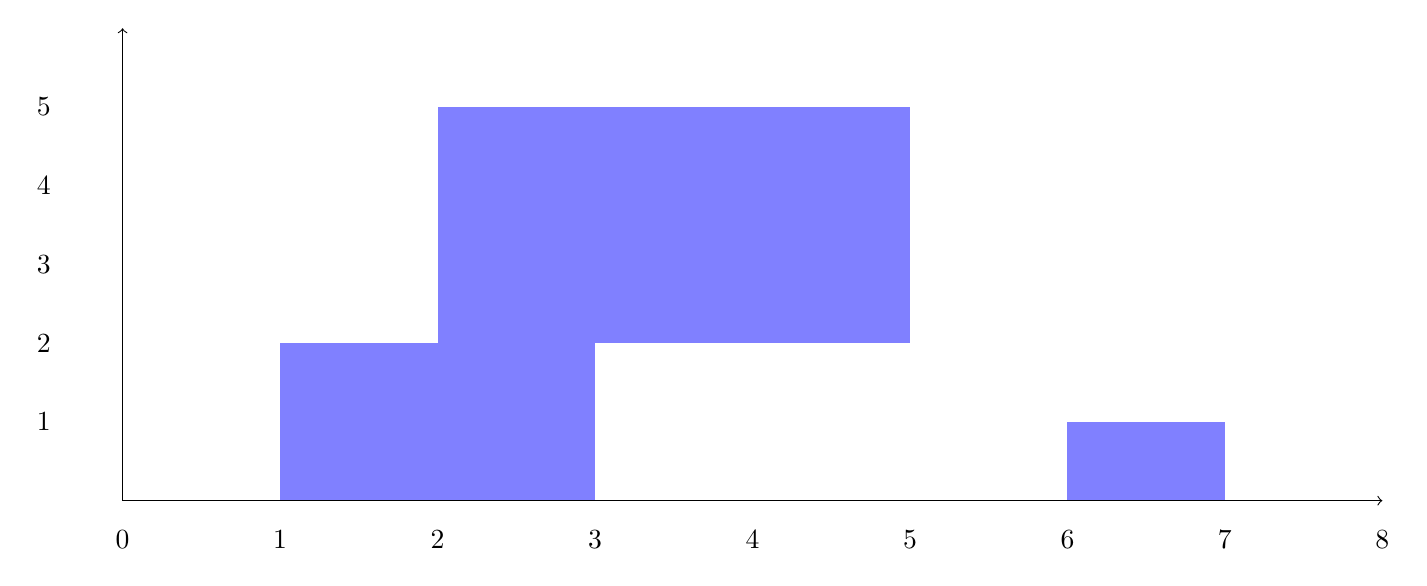
\begin{tikzpicture}
\fill[color=blue!50] (13,0.5cm) rectangle ++(2,1cm);
\fill[color=blue!50] (5,2.5cm) rectangle ++(6,3cm);
\fill[color=blue!50] (3,0.5cm) rectangle ++(4,2cm);
\draw[->] (1,0.5cm) -- ++(16,0);
\draw[->] (1,0.5cm) -- ++(0,6cm);
\foreach \x / \y in {1/0,3/1,5/2,7/3, 9/4, 11/5, 13/6, 15/7, 17/8}
\node (\x) at (\x, 0) {$\y$};
\foreach \x / \y in {1.5cm/1, 2.5cm/2, 3.5cm/3, 4.5cm/4, 5.5cm/5}
\node (\x) at (0, \x) {$\y$};
\end{tikzpicture}

The maximum height of any square is still 5.

Thus, we return an answer of \lstinline[language=C++, basicstyle=\small\ttfamily, keywordstyle=\bfseries\color{green!40!black}]|[2, 5, 5]|.
\end{flushleft}

\paragraph{Example 2:}
\begin{flushleft}
\textbf{Input}: \lstinline[language=C++, basicstyle=\small\ttfamily, keywordstyle=\bfseries\color{green!40!black}]|[[100, 100], [200, 100]]|

\textbf{Output}: \lstinline[language=C++, basicstyle=\small\ttfamily, keywordstyle=\bfseries\color{green!40!black}]|[100, 100]|

\textbf{Explanation}: Adjacent squares do not get stuck prematurely - only their bottom edge can stick to surfaces.
\end{flushleft}

\paragraph{Note:}
\begin{itemize}
\item The number of total squares is in range $(1, 1000)$

\item The bottom left of each square is in range $(1,,10^8)$.

\item The side length of each square is  in range $(1,10^6)$.
\end{itemize}

\subsection{Offline Propagation}
Suppose $F[i]$ be the maximum height of the interval specified by \lstinline[language=C++, basicstyle=\small\ttfamily, keywordstyle=\bfseries\color{green!40!black}]|positions[i]|. At the end, we'll return a running max of $F$.

For each square \lstinline[language=C++, basicstyle=\small\ttfamily, keywordstyle=\bfseries\color{green!40!black}]|positions[i]|, the maximum height will get higher by the size of the square we drop. Then, for any future squares that intersect the interval \lstinline[language=C++, basicstyle=\small\ttfamily, keywordstyle=\bfseries\color{green!40!black}]|[left, right)| (where \lstinline[language=C++, basicstyle=\small\ttfamily, keywordstyle=\bfseries\color{green!40!black}]|left = positions[i][0]|, \lstinline[language=C++, basicstyle=\small\ttfamily, keywordstyle=\bfseries\color{green!40!black}]|right = positions[i][0] + positions[i][1]|), we'll update the maximum height of that interval.

\setcounter{lstlisting}{0}
\begin{lstlisting}[style=customc, caption={Offline Propagation}]
vector<int> fallingSquares( vector<vector<int>>& positions )
{
    auto& S = positions;

    //H[i] is the highest
    //height in the range of (S[i][0], S[i][0]+S[i][1])
    vector<int> H( S.size(), 0 );

    for( size_t i = 0; i < S.size(); ++i )
    {
        int range_l = S[i][0];
        int side = S[i][1];
        int range_r = range_l + side;

        //square S[i] is dropped
        //but H[i] does not add its side length
        //thus we need to increment
        //the maximum height in the range
        //of S[i] by the side length.
        H[i] += side;

        for( size_t j = i + 1; j < S.size(); ++j )
        {
            int left = S[j][0];
            int right = S[j][0] + S[j][1];

            if( ( left < range_r ) && ( range_l < right ) )
            {
                //S[j] is overlapped with S[i]
                //we update the maximum length
                //that could be affected by H[i]
                H[j] = ( max )( H[j], H[i] );
            }
        }
    }

    //we need to get
    //the running maximum H
    //as the answer
    vector<int> ans;
    ans.reserve( H.size() );

    int curH = -1;

    for( int h : H )
    {
        curH = ( max )( h, curH );
        ans.push_back( curH );
    }

    return ans;
}
\end{lstlisting}

\subsection{Brute Force with Coordinate Compression}
Since the range left and right ends are limited, we can use a technique called \textbf{coordinate compression} to map these points to adjacent integers. This technique requires a set $S$ and a hash map $M$. Since set can sort the points when inserting, we can get sorted coordinates when iterating through the set $S$.

In this approach, we compress the positions and then for each current square, we first get the maximum height from the range that current square covers, and then update the maximum heights inside this range. To achieve this, we make use of an array $H$ to save maximum height of the interval specified by each square.

\begin{lstlisting}[style=customc, caption={Coordinate Compression}]
vector<int> fallingSquares( vector<vector<int>>& positions )
{
    //compress coordinates
    set<int> coords;

    for( const auto& square : positions )
    {
        coords.insert( square[0] );
        coords.insert( square[0] + square[1] - 1 );
    }

    unordered_map<int, int> m_index;
    int index = 0;

    //map each coord
    //to a continuous integer
    for( int coord : coords )
    {
        m_index.emplace( coord, index++ );
    }

    vector<int> ans;
    ans.reserve( positions.size() );

    vector<int> H( index, 0 );

    int best = 0;

    for( const auto& sq : positions )
    {
        //get the coord index
        int left = m_index[sq[0]];
        int right = m_index[sq[0] + sq[1] - 1];

        //query the maximum height in [left, right]
        int max_h = 0;
        for( int i = left; i <= right; ++i )
        {
            max_h = ( max )( max_h, H[i] );
        }

        //increase the height by the side length
        //of current square
        max_h += sq[1];

        //update maximum height in [left, right]
        for( int i = left; i <= right; ++i )
        {
            H[i] = ( max )( H[i], max_h );
        }

        best = ( max )( best, max_h );
        ans.push_back( best );
    }

    return ans;
}
\end{lstlisting}

\subsection{Segment Tree With Lazy Propagation}
Since we are querying maximum heights in a range, segment tree would be another suitable approach. In this approach, the merge function will get the maximum height from the merged two intervals.

The working flow is same as last approach
\begin{enumerate}
\item Query the maximum height in the range specified by current square.
\item Update the maximum heights in this range.
\item Save running maximum height to the output.
\end{enumerate}

\begin{lstlisting}[style=customc, caption={Segment Tree}]
struct STree
{
    vector<int> tree;
    vector<int> lazy;

    STree( int sz )
        : tree( sz, 0 )
        , lazy( sz, 0 )
    {
    }

    void lazy_prop( int ti, int a_start, int a_end )
    {
        if( lazy[ti] )
        {
            //node tree[ti] has pending updates
            tree[ti] = ( max )( tree[ti], lazy[ti] );

            if( a_start != a_end )
            {
                lazy[2 * ti + 1] = ( max )( lazy[2 * ti + 1], lazy[ti] );
                lazy[2 * ti + 2] = ( max )( lazy[2 * ti + 2], lazy[ti] );
            }

            lazy[ti] = 0;
        }
    }

    bool check_range( int a_start, int a_end, int q_start, int q_end )
    {
        if( a_start > a_end )
        {
            return false;
        }

        if( ( a_start > q_end ) || ( a_end < q_start ) )
        {
            //cover range [a_start, a_end] does not
            //overlap with query range [q_start, q_end]
            return false;
        }

        return true;
    }

    bool is_inside_query( int a_start, int a_end, int q_start, int q_end )
    {
        if( ( a_start >= q_start ) && ( a_end <= q_end ) )
        {
            //cover range [a_start, a_end] is completely inside
            //query range [q_start, q_end]
            return true;
        }

        return false;
    }

    int query( int ti, int a_start, int a_end, int q_start, int q_end )
    {
        lazy_prop( ti, a_start, a_end );

        if( !check_range( a_start, a_end, q_start, q_end ) )
        {
            //either invalid cover range
            //or not overlap with query range
            return 0;
        }

        if( is_inside_query( a_start, a_end, q_start, q_end ) )
        {
            //cover range is completely inside query range
            return tree[ti];
        }

        //cover range is overlapped with query range
        int mid = ( a_start + a_end ) / 2;

        //left result
        int res_l = query( 2 * ti + 1, a_start, mid, q_start, q_end );
        //right result
        int res_r = query( 2 * ti + 2, mid + 1, a_end, q_start, q_end );

        return ( max )( res_l, res_r );
    }

    void update( int ti, int a_start, int a_end, int q_start, int q_end, int value )
    {
        lazy_prop( ti, a_start, a_end );

        if( !check_range( a_start, a_end, q_start, q_end ) )
        {
            //either invalid cover range
            //or not overlap with query range
            return;
        }

        if( is_inside_query( a_start, a_end, q_start, q_end ) )
        {
            //cover range is completely inside query range
            tree[ti] = ( max )( tree[ti], value );

            //put impending update to lazy array
            if( a_start != a_end )
            {
                lazy[2 * ti + 1] = ( max )( lazy[2 * ti + 1], value );
                lazy[2 * ti + 2] = ( max )( lazy[2 * ti + 2], value );
            }
        }
        else
        {
            int mid = ( a_start + a_end ) / 2;
            //update left
            update( 2 * ti + 1, a_start, mid, q_start, q_end, value );
            //update right
            update( 2 * ti + 2, mid + 1, a_end, q_start, q_end, value );

            //update current node
            tree[ti] = ( max )( tree[2 * ti + 1], tree[2 * ti + 2] );
        }
    }
};


vector<int> fallingSquares( vector<vector<int>>& positions )
{

    //coordinat compression
    set<int> coords;

    for( const auto& p : positions )
    {
        coords.insert( p[0] );
        coords.insert( p[0] + p[1] - 1 );
    }

    unordered_map<int, int> m_index;

    int N = 0;

    for( int coord : coords )
    {
        m_index.emplace( coord, N++ );
    }

    int h_tree = 1;

    while( ( 1 << h_tree ) < N )
    {
        ++h_tree;
    }

    int tree_size = ( 1 << h_tree ) * 2;


    //create segement tree
    STree stree( tree_size );


    int best = 0;
    vector<int> ans( positions.size() );

    int i_ans = 0;

    for( const auto& p : positions )
    {
        int left = m_index[p[0]];
        int right = m_index[p[0] + p[1] - 1];

        //the query is starting from the root
        //ti=0, and cover range is [0, N-1]
        int h = stree.query( 0, 0, N - 1, left, right );
        //increase h by current square side length
        h += p[1];

        //update in range [left, right]
        //starting from the root ti=0, and cover range
        //is [0, N-1]
        stree.update( 0, 0, N - 1, left, right, h );

        best = ( max )( best, h );

        ans[i_ans++] = best;
    }

    return ans;
}
\end{lstlisting}